% Font size, paper type
\documentclass[12pt]{article}
% Aesthetic margins
\usepackage[margin=1in]{geometry}
% Core math packages,
% Mathtools loads amsmath, and amsmath gives basic math symbs
% Amsfonts & amssymb are misc. symbols you might need
\usepackage{mathtools, amsfonts, amssymb}
% Links in a pdf
\usepackage{hyperref}
% Use in pictures, graphs, and figures
\usepackage{graphicx}
% Header package
\usepackage{fancyhdr}
% Underlining with line breaks
\usepackage{ulem}
% Adjust accordingly given warning messages
\setlength{\headheight}{15pt}
% So we can more easily format text with pictures
\usepackage{float}

% Sets footer
\pagestyle{fancy}
% Removes default footer style
\fancyhf{}

\rhead{
  Shengdong Li
  Calc 3
}

\rfoot{
  Page \thepage
}

% Makes links look more appealling
\hypersetup{
    colorlinks=true,
    linkcolor=blue,
    filecolor=magenta,      
    urlcolor=cyan,
}

% \usepackage{indentfirst}

\begin{document}
\title{Problem 2 = $\int_{0}^{1}xe^{-x^{3}}dx$}
\author{by Shengdong Li}
\date{5 December 2020}
\maketitle

Hello William, 
Deepest of apologies for my confusion with what was problem 1 and what was problem 2. 

You said that my step size of $\frac{1}{4}$ was smaller and therefore more innacurate than Kate's step size of $\frac{1}{8}$, and I definitely agree with that comment. However, another thing that I also noticed was that the terms of the Riemann sums are a lot easier to calculate than Taylor, and so we could've easily increased the $n$ value slightly more. 

With that being said, below I have redone my initial post working through problem 2 instead.

\section{Taylor Series Approximation}
\begin{align}
  \intertext{I chose to center the Taylor series for this function at $0$, since we could then use Maclaurin shortcuts knowing the summation representation of $e^x$}
  e^{x}                              & =\sum_{n=0}^{\infty}\frac{x^{n}}{n!}                                                                                                                                     \\
  \intertext{Now we can plugin $-x^3$ for $x$, and multiply the $x$}
  xe^{-x^{3}}                        & =x\sum_{n=0}^{\infty}\frac{\left(-x^{3}\right)^{n}}{n!}                                                                                                                  \\
  xe^{-x^{3}}                        & =x\sum_{n=0}^{\infty}\frac{\left(-1\right)^{n}\cdot x^{3n}}{n!}                                                                                                       \\
  xe^{-x^{3}}                        & =\sum_{n=0}^{\infty}\frac{\left(-1\right)^{n}\cdot x^{3n+1}}{n!}                                                                                                         \\
  \intertext{Next, I chose to go to the fourth degree Taylor polynomial, since by the formula it would have $2$ terms and it wouldn't be impossible to calculate by hand}
  T_{4}\left(x\right)                & =\frac{\left(-1\right)^{\left(0\right)}\cdot x^{3\left(0\right)+1}}{\left(0\right)!}+\frac{\left(-1\right)^{\left(1\right)}\cdot x^{3\left(1\right)+1}}{\left(1\right)!} \\
                                     & =x-x^{4}                                                                                                                                                                 \\
  \intertext{We need to integrate this polynomial from $0$ to $1$}
  \int_{0}^{1}\left(x-x^{4}\right)dx & =\left[\frac{x^{2}}{2}-\frac{x^{5}}{5}\right]_{0}^{1}                                                                                                                    \\
                                     & =\left(\frac{1}{2}-\frac{1}{5}\right)-\left(\frac{0}{2}-\frac{0}{5}\right)                                                                                               \\
                                     & =\frac{1}{2}-\frac{1}{5}                                                                                                                                                 \\
                                     \Aboxed{& =\frac{3}{10}}                                                                                                                                                            
\end{align}
\section{Riemann Sums Approximation}
\begin{align}
  \intertext{For Riemann sums, I chose to go for Simpson's with $n=4$, matching the degree of the Taylor polynomial}
  \Delta x                & =\frac{1-0}{4}=\frac{1}{4}                                                                                                                                               \\
  S_{4}                              & =\frac{\left(\frac{1}{4}\right)}{3}\left(f\left(0\right)+4f\left(\frac{1}{4}\right)+2f\left(\frac{1}{2}\right)+4f\left(\frac{3}{4}\right)+f\left(1\right)\right)         \\
                                     & =\frac{1}{12}\left(\left(0\right)+4\left(.25\right)+2\left(.441\right)+4\left(.492\right)+\left(.368\right)\right)                                                       \\
                                     \Aboxed{& =.3515}                                                                                                                                                                   
\end{align}

\section{Observations}
Comparing the results, the difference between the two methods was very small, with the results being $.0515$ within each other. On the other hand, counting the terms, $T_4(x)$ of $\int_{0}^{1}xe^{-x^{3}}dx$ only had $2$ terms, while Riemann had a full $5$ strips, so just looking at these results Riemann might be slightly more accurate.

The graphs of the two functions confirms Riemann being much more accurate than Taylor.
\begin{figure}[H]
  \begin{center}
    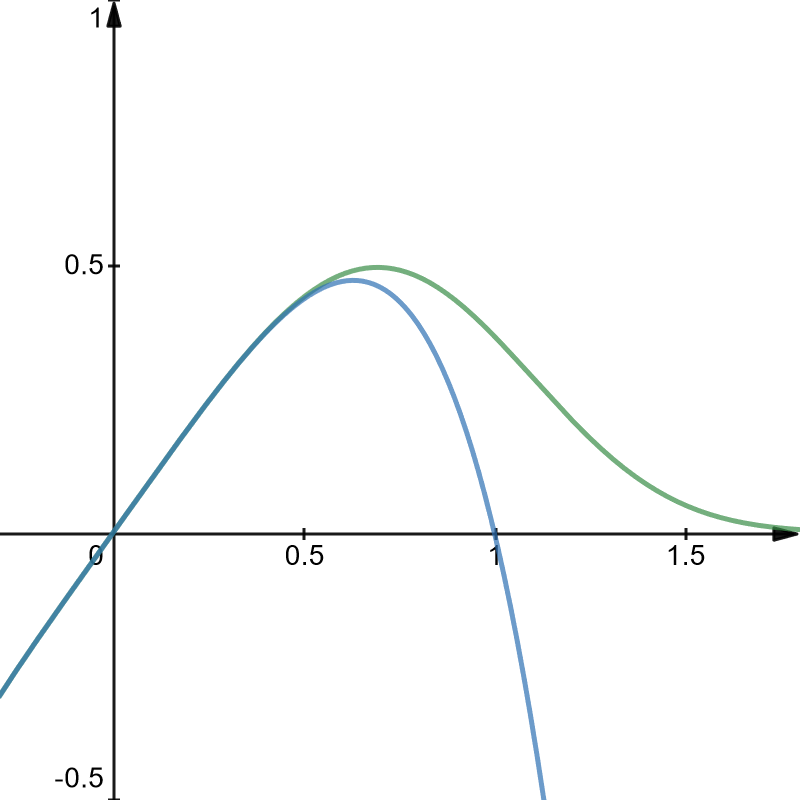
\includegraphics[scale=.3]{taylor.png}
    \caption{\textit{Picture of taylor function.} Desmos link \href{https://www.desmos.com/calculator/zhjxfaf7nq}{\textcolor{blue}{here}}}
  \end{center}
\end{figure}

\begin{figure}[H]
  \begin{center}
    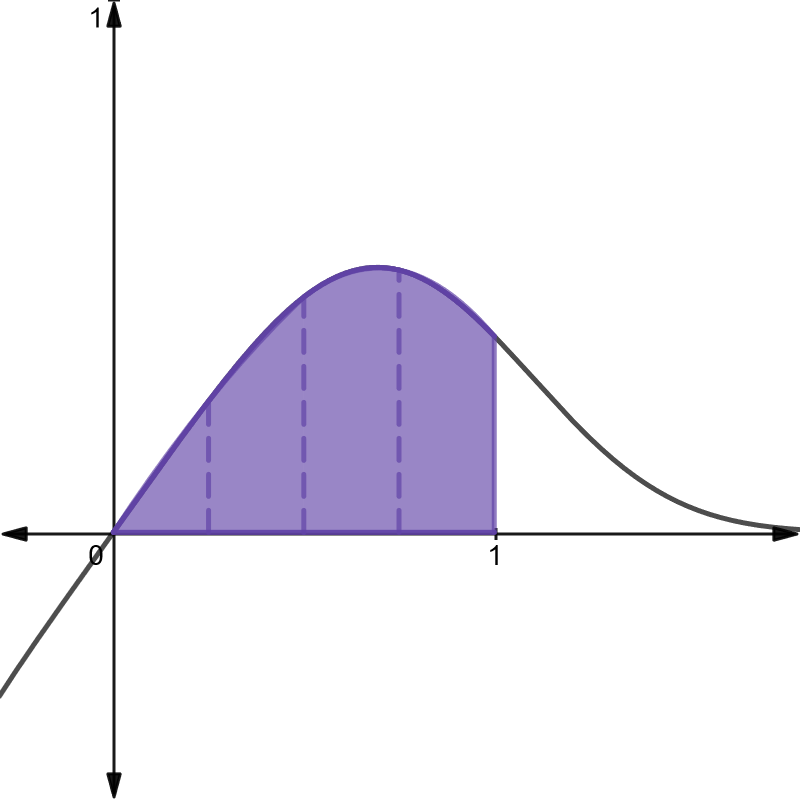
\includegraphics[scale=.3]{riemann.png}
    \caption{\textit{Picture of riemann sum.} Desmos link \href{https://www.desmos.com/calculator/vytmchsw3b}{\textcolor{blue}{here}}}
  \end{center}
\end{figure}

It is clear looking at the graph of these two approximations that the taylor function drops off sharply while the Simpson's Riemann Sums almost matches the function exactly. If we kept going past $1$ and expanded the bounds from $0$ to $2$, then the taylor representation would be exponentially worse and much more inaccurate compared to Simpson's.

Therefore, Taylor series might be good for small bounds where the taylor polynomial can match the curve, but for large bounds Riemann's sum not even necessarily using Simpson's would be much more accurate!

% Remember to use \ldots
\end{document}